\subsection{Evaluation of object lists - Post processing}

After recording object list data streams in Rosbag files there is the possibility to analyse data in different ways by the post processing application offline. The user can either analyse single data streams or compare two different ones. An essential usage would be the comparison of a simulation data stream (Ground-Truth data) to a sensor data stream (camera data). The post processing application provides the opportunity to display several data values within the recorded Rosbag file relating to contained message frames.

\subsubsection{Basic analysis}

Considered to one single Rosbag file specific attribute values of single objects which are selected by their object ID can be displayed. The variety of available attribute types is shown in table 
%\ref{<Object list – attributes table (TP1)>}
. In addition, the number of detected objects can be visualized. 

\subsubsection{Advanced analysis}

Regarding two Rosbag recordings further analysis methods for comparing the streams are provided. In this case a common time base needs to be generated. To avoid errors because of time variation of both recordings following mapping algorithm is executed. Each frame time stamp is handled as time relative to its Rosbag start time in milliseconds. To every frame in the Rosbag file which is provided by sensor data a frame of simulation data is dedicated. The simulation frame to choose is the latest past frame in relative stream time. The principle of frame mapping is shown in figure \ref{fig:frame_mapping}. With this mechanism pairs of frames are generated (sensor frame with corresponding simulation frame).

\begin{figure}[thpb]
	\centering
	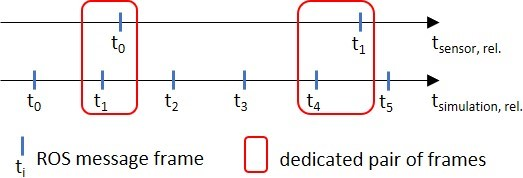
\includegraphics[width=\linewidth]{images/frame_mapping.pdf}
	\caption{Principle of frame mapping algorithm}
	\label{fig:frame_mapping}
\end{figure}

A fundamental use case in analysing the recorded Rosbag files is to evaluate the quality of sensor data. Therefore, it is necessary to operate the mapping of object detection by the sensor in comparison to the simulation data. For this purpose, the algorithm \textbf{Intersection over Union} is applied.

%\include{<Intersection_over_Union (Max H.)>}

!! Put part of Max H. (IoU) here !!

As a result of object mapping it is possible to visualize the number of True Positive (TP), False Positive (FP), False Negative (FN) and mismatch (mm) cases per frame. Further, following quality of service parameter according to \cite{Reway.2018} can be displayed:

\begin{itemize}
	
	\item recall per frame
	\item precision per frame
	\item FPPI per data stream (sensor)
	\item MOTA per data stream (sensor)
	\item MOTP per data stream (sensor)
	
\end{itemize}

Another feature of the post processing application is the analysis of deviations by calculating differences of specific attribute values between two recorded data streams. For that matter only True Positive cases in object mapping are regarded and the concerning object is selected by its object ID in the simulation data record. The difference value results from

$$
difference = value_{simulation} - value_{sensor} \eqno{(???)}
$$

On top of every post processing analysis - except from FPPI, MOTA and MOTP - the mean value and standard deviation of the corresponding value series are calculated.

\subsection{Visualization of object lists(TP3)}

The published topics of Ground-Truth data and Camera-Calculation data will be subscribed. Each topic contains the ego vehicle data and the specific generated object list. In order to evaluate the object lists, the objects will be analyzed per frame. In RVIZ, the objects are represented by primitive figures with the help of marker messages.



Marker messages are described with specific properties such as position, scale, type, color, orientation. Each object class will assigned selected shapes and colors so that they can be differentiate in RVIZ. The display variants for the possible object classes are shown in table \ref{ClassificationAssignment}. 

\begin{table}[h]
	\caption{Classification Assignment}
	\label{ClassificationAssignment}
	\begin{center}
		\begin{tabular}{c c c}
			\hline
			Classification & Shape & Color[RGB]\\
			\hline
			car & cube & [1, 0, 0]\\
			truck & cube & [0, 1, 0]\\
			pedestrian & cylinder & [0, 0, 1]\\
			motorcyle & cube & [1, 0, 1]\\
			car & cube & [1, 0, 0]\\
			bicycle & cylinder & [1, 1, 0]\\
			stacionary & sphere & [0, 1, 1]\\
			other & sphere & [1, 1, 1]\\
			\hline
			
			
		\end{tabular}
	\end{center}
\end{table}

In addition, the yaw angle of the objects has to be transformed into a quaternion for the visualization in RVIZ. The markers for the calculated camera data are assigned an RGB alpha value of 0.5, so that the difference between the camera data and the GT data is visually recognizable. 

<<<<<<< HEAD
The highest detection probability of an object indicates the classification, so that the properties value of each shape can assigned to the marker message. Furthermore, each detection position must be mirrored on the Y-axis, because the vehicle coordinate system does not match to the RVIZ coordinate system. Finally, the generated markers are combined into a marker array and will be published.
=======



The highest detection probability of an object indicates the classification, so that the properties value of each shape can be assigned to the marker message. Furthermore, each detection position must be mirrored on the Y-axis, because the vehicle coordinate system does not match to the RVIZ coordinate system. Finally, the generated markers are combined into a marker array and will be published.
>>>>>>> 0ac92cd024158a65a574cf276325f8ba7c4b1260

The published topics of Ground-Truth data, camera data and ego vehicle data are also saved in a Rosbag file. Each Rosbag file contains the published ego data and the corresponding object lists. In the following, these files are used for post processing.